\Variant{01.12.2024 (1-smena)}
\QQ{1}{$\overline{2023ab}$ körinişidagi olti xonali sonlar orasida $36$ ga qoldiqsiz bölinadiganlari neçta?
\Opts{$3$ ta}{$2$ ta}{$1$ ta}{Mavjud emas}}
\QQ{2}{Hisoblang: \ $4{,}(36):3{,}1(9)+\dfrac1{3\frac17}$
\Opts{$\dfrac{35}{22}$}{$1\dfrac{15}{22}$}{$\dfrac{17}{35}$}{$2\dfrac5{22}$}}
\QQ{3}{Kema daryo oqimi böyiça harakatlanib $S$ masofaga $80$ daqiqa vaqt sarflaydi. Oqimga qarşi harakatlanib $S$ masofaning yarmini $60$ daqiqada bosib ötadi. Kemaning tezligi oqim tezligidan neça marta katta?
\Opts{$6$}{$7$}{$4$}{$5$}}
\QQ{4}{Bir oilaning oylik maoşi $15\,000\,000$ söm. Uning $60\%$i oilaviy harajatlarga sarflanar edi. Qolgan pulning $30\%$ini bankka omonatga qöyadi. Oila bankka neça söm pul qöygan?
\Opts{$1\,800\,000$}{$2\,000\,000$}{$2\,500\,000$}{$2\,200\,000$}}
\QQ{5}{$x+y=10^z$, $x^2+y^2=10^{z+1}$, $x^3+y^3=a\cdot10^{3z}+b\cdot10^{2z}$ bölsa, $a$ va $b$ ning ratsional qiymatlari yiğindisini toping.
\Opts{$15{,}5$}{$16{,}5$}{$18{,}5$}{$14{,}5$}}
\QQ{6}{Hisoblang:
\[\frac1{2\sqrt6+5}-5+2\sqrt6\]
\Opts{$4\sqrt6$}{$10$}{$0$}{$3\sqrt6$}}
\QQ{7}{Hisoblang:
\[\sqrt{21-12\sqrt3}\cdot\sqrt{\left(\sqrt3-4\right)^2}\]
\Opts{$11\sqrt3-18$}{$14\sqrt3-17$}{$15+7\sqrt3$}{$18-11\sqrt3$}}
\QQ{8}{Arifmetik progressiyada $a_1+a_3+a_5+\dots+a_{2n-1}=96$; \ $a_{n-2}+a_{n+2}=12$ bölsa, $n$ ning qiymatini toping.
\Opts{$8$}{$32$}{$24$}{$16$}}
\QQ{9}{Çeksiz kamayuvçi geometrik progressiyaning yiğindisi $22{,}5$ ga, dastlabki ikkita hadi yiğindisi $20$ ga va $0<q<1$ bölsa, progressiyaning törtinçi hadini toping.
\Opts{$\dfrac5{18}$}{$1$}{$\dfrac58$}{$\dfrac59$}}
\QQ{10}{$a=2024$ va $b=2023$ bölsa, $a^3-b^3+a^2+b^2+2-5ab$ ning qiymatini toping.
\Opts{$4$}{$1$}{$-1$}{$0$}}
\QQ{11}{Agar $x+y=3$, $x\cdot y=-1$ bölsa, $\dfrac{x(y+1)^2-y(x+1)^2}{x^2(y+1)-y^2(x+1)}$ ni toping.
\Opts{$-1$}{$0$}{$1$}{$10$}}
\QQ{12}{$12345''$ ni gradusda, minutda, sekundda ifodalang.
\Opts{$3^\circ25'45''$}{$3^\circ45'55''$}{$4^\circ25'45''$}{$4^\circ26'45''$}}
\QQ{13}{Soddalaştiring:
\[\frac{2\sin^2x\cos^4x-2\sin^4x\cos^2x}{1-\cos^24x\sin^24x-\cos^44x}\]
\Opts{$\dfrac1{8\cos2x}$}{$\dfrac1{2\cos2x}$}{$1$}{$\dfrac1{\cos2x}$}}
\QQ{14}{$16^{\frac1x}-20\cdot2^{\frac2x-2}+4=0$ tenglamaning haqiqiy ildizlari neçta?
\Opts{$3$ ta}{$1$ ta}{$2$ ta}{$4$ ta}}
\QQ{15}{$\sqrt{\log_x\sqrt{4x}}=-\dfrac1{\log_4x}$ tenglamaning haqiqiy ildizlari köpaytmasini toping (agar u bitta bölsa, şu ildizini toping).
\Opts{$\dfrac1{16}$}{$\dfrac14$}{$\dfrac12$}{$2$}}
\QQ{16}{$|3x+6|=15$ tenglamaning haqiqiy ildizlari köpaytmasini toping. (Agar u bitta bölsa, şu ildizini toping)
\Opts{$-21$}{$-7$}{$-5$}{$0$}}
\QQ{17}{$\dfrac{x^2+4}{x+2\sqrt x+2}=\dfrac{x^2-5x+4}{x+3\sqrt x+2}$ tenglamaning haqiqiy ildizlari yiğindisini toping. (Agar u bitta bölsa, şu ildizini toping)
\Opts{$1$}{$0$}{$-1$}{Yeçimga ega emas}}
\QQ{18}{$2\sqrt{x-3}>x-6$ tengsizlikni qanoatlantiruvçi barça butun sonlar yiğindisini toping.
\Opts{$56$}{$63$}{$74$}{$81$}}
\QQ{19}{$\sqrt{x^2-6x+9}\cdot\sqrt{-x^2+3x+10}>0$ tengsizlikni qanoatlantiruvçi butun sonlar neçta?
\Opts{$5$ ta}{$6$ ta}{Çeksiz köp}{$8$ ta}}
\QQ{20}{$f(x)=\dfrac{\sqrt{-x^2+3x+10}}{\left|1-\log_x2\right|\left(\sin x-\frac\pi3\right)}$ funksiyaning aniqlaniş sohasiga tegişli neçta butun son bor?
\Opts{$5$ ta}{$6$ ta}{$7$ ta}{$3$ ta}}
\QQ{21}{Aniqmas integralni toping.
\[\int\frac{\ln\ln x}x\,dx\]
\Opts{$\ln x\left(\ln\ln x-1\right)+C$}{$\ln x\left(\ln\ln x+1\right)+C$}{$\ln\ln x+C$}{$\ln x+C$}}
\QQ{22}{$f(x)=\sin^3\dfrac x2$ bölsa, $f'\left(\dfrac{2\pi}3\right)$ ni toping.
\Opts{$\dfrac9{16}$}{$\dfrac98$}{$\dfrac7{15}$}{$\dfrac57$}}
\QQ{23}{$ABCD$ törtburçakka aylana içki çizilgan. $AB=CD=7$ va $AD=6$ bölsa, $BC$ ni toping.
\qfig{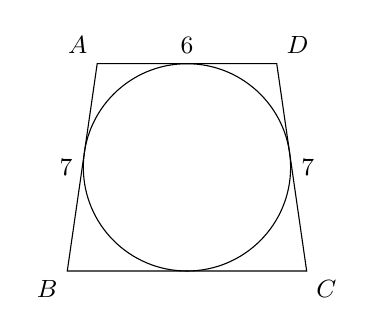
\begin{tikzpicture}[scale=0.38,font=\small]
\coordinate (B) at (0,0); \coordinate (C) at (8,0); \coordinate (D) at (7,6.928); \coordinate (A) at (1,6.928);
\draw (A)--(B)--(C)--(D)--cycle; \draw (4,3.464) circle (3.464);
\node[above left] at (A) {$A$}; \node[below left] at (B) {$B$}; \node[below right] at (C) {$C$}; \node[above right] at (D) {$D$};
\node[left] at (0.5,3.46) {$7$}; \node[right] at (7.5,3.46) {$7$}; \node[above] at (4,6.928) {$6$};
\end{tikzpicture}}
\Opts{$6$}{$8$}{$14$}{$15$}}
\QQ{24}{$ABC$ teng yonli uçburçakka aylana içki çizilgan, $AB=AC$. Aylana uriniş nuqtasidan $AB$ tomonni $6$ va $4$ ga teng kesmalarga ajratdi ($AB>BC$). $ABC$ uçburçakning yuzini toping.
\qfig{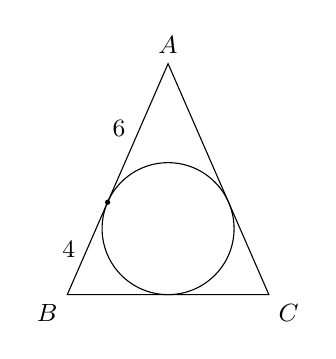
\begin{tikzpicture}[scale=0.32,font=\small]
\coordinate (B) at (-4,0); \coordinate (C) at (4,0); \coordinate (A) at (0,9.165); \coordinate (K) at (-2.4,3.666);
\draw (A)--(B)--(C)--cycle; \draw (0,2.619) circle (2.619); \fill (K) circle (3pt);
\node[above] at (A) {$A$}; \node[below left] at (B) {$B$}; \node[below right] at (C) {$C$};
\node[left] at (-1.3,6.6) {$6$}; \node[left] at (-3.3,1.8) {$4$};
\end{tikzpicture}}
\Opts{$96$}{$10\sqrt{21}$}{$48$}{$8\sqrt{21}$}}
\QQ{25}{$A$ dan $B$ gaça bölgan eng qisqa masofani toping.
\qfig{\begin{tikzpicture}[scale=1.25,font=\small]
\coordinate (B) at (0,0); \coordinate (C) at (4.24,0); \coordinate (A) at (4.95,0.707);
\draw (B)--(C)--(A); \fill (A) circle (1.2pt); \fill (B) circle (1.2pt); \fill (C) circle (1.2pt);
\draw ($(C)+(45:0.3)$) arc (45:180:0.3);
\node[below] at (B) {$B$}; \node[below] at (C) {$C$}; \node[right] at (A) {$A$};
\node[below] at (2.12,0) {$15\sqrt2$}; \node[below right] at (4.6,0.35) {$5$}; \node at (3.95,0.55) {$135^\circ$};
\end{tikzpicture}}
\Opts{$25$}{$15$}{$10$}{$10\sqrt2$}}
\QQ{26}{$ABCD$ parallelogrammda $BC$ tomonda $E$ nuqta, $AD$ tomonda $F$ nuqta olingan. $EF$ va $AC$ kesmalar $P$ nuqtada kesişadi. $AD=4AF$, $AC=3AP$. $ABEP$ törtburçakning yuzi $16$ ga teng bölsa, ştrixlangan soha yuzini toping.
\qfig{\begin{tikzpicture}[scale=0.85,font=\small]
\coordinate (A) at (0,0); \coordinate (D) at (4,0); \coordinate (B) at (1,2.6); \coordinate (C) at (5,2.6); \coordinate (F) at (1,0); \coordinate (P) at (1.667,0.867); \coordinate (E) at (3,2.6);
\fill[qfill] (P)--(F)--(D)--(C)--cycle;
\draw (A)--(B)--(C)--(D)--cycle; \draw (A)--(C); \draw (F)--(E);
\node[below left] at (A) {$A$}; \node[above left] at (B) {$B$}; \node[above right] at (C) {$C$}; \node[below] at (D) {$D$}; \node[below] at (F) {$F$}; \node[above] at (E) {$E$}; \node[above left] at (P) {$P$};
\end{tikzpicture}}
\Opts{$22$}{$21$}{$20$}{$23$}}
\QQ{27}{$y=x^2-\sqrt{9+x^2}$ funksiyaning eng kiçik butun qiymatini toping.
\Opts{$-3$}{$1$}{$0$}{$3$}}
\QQ{28}{$ABCDEFHI$ muntazam sakkizburçak va $AGJKI$ muntazam beşburçak berilgan. Bunga köra $\angle BAG$ burçakni toping.
\qfig{\begin{tikzpicture}[scale=0.62,font=\small]
\coordinate (A) at (0,0); \coordinate (I) at (2,0); \coordinate (H) at (3.414,1.414); \coordinate (F) at (3.414,3.414); \coordinate (E) at (2,4.828); \coordinate (D) at (0,4.828); \coordinate (C) at (-1.414,3.414); \coordinate (B) at (-1.414,1.414);
\coordinate (G) at (-0.618,1.902); \coordinate (K) at (2.618,1.902); \coordinate (J) at (1,3.078);
\draw (A)--(I)--(H)--(F)--(E)--(D)--(C)--(B)--cycle; \draw (A)--(G)--(J)--(K)--(I);
\draw ($(A)!0.45cm!(B)$) arc [start angle=135,end angle=108,radius=0.45cm];
\node[below] at (A) {$A$}; \node[below] at (I) {$I$}; \node[right] at (H) {$H$}; \node[right] at (F) {$F$}; \node[above] at (E) {$E$}; \node[above] at (D) {$D$}; \node[left] at (C) {$C$}; \node[left] at (B) {$B$};
\node[left] at (G) {$G$}; \node[right] at (K) {$K$}; \node[above] at (J) {$J$};
\end{tikzpicture}}
\Opts{$27^\circ$}{$36^\circ$}{$54^\circ$}{$20^\circ$}}
\QQ{29}{$ABCD$ töğri törtburçakning $A$ uçi koordinatalar boşida, $B$ uçi $Ox$ öqida. $C$ uçining koordinatasi $(5;\,4)$ va $\dfrac12\overrightarrow{BE}=\overrightarrow{BC}$ bölsa, $ABED$ törtburçakning yuzini toping.
\Opts{$20$}{$15$}{$30$}{$40$}}
\QQ{30}{Tekislikda yotmagan $A$ nuqta orqali tekislikka $AH$ balandlik va $AM$ oğma tuşirilgan. Agar oğma va tekislik orasidagi burçak $37^\circ$ va $AH=6$ bölsa, $H$ uçidan $AM$ oğmagaça bölgan eng qisqa masofani toping. ($\cos37^\circ=0{,}8$ deb oling)
\Opts{$1{,}8$}{$3{,}6$}{$4{,}8$}{$2{,}4$}}
\QQ{31}{$A=\{x\mid-3\le x<5;\ x\in\mathbb Z\}$, $B=\{x\mid-5\le x<3;\ x\in\mathbb Z\}$, $C=\{x\mid-4\le x<6;\ x\in\mathbb Z\}$, $D=\{x\mid-3\le x<7;\ x\in\mathbb Z\}$ bölsa, $(A\cup C)'\cap(B\cup D)$ ning qism töplamlari sonini toping.
\Opts{$2$}{$16$}{$8$}{$4$}}
\QQ{32}{Tört xonali sonlar içidan raqamlari toq sonlardan iborat bölgan va $5$ ga karrali son böliş ehtimolligini toping.
\Opts{$\dfrac1{72}$}{$\dfrac1{36}$}{$\dfrac1{108}$}{$\dfrac15$}}
\QQ{33}{\Moslash{Diametri $10$ cm ga teng bölgan ikkita bir xil silindr berilgan. Silindrdan kesim kesib olib tirsak yasaldi. ($\pi\approx3$ deb oling)
\par\centering\begin{tikzpicture}[scale=0.13,font=\scriptsize]
\begin{scope}
\draw (0,0) ellipse (1.6 and 5); \draw (0,5)--(20,5); \draw (0,-5)--(20,-5); \draw (20,-5) arc (-90:90:1.6 and 5);
\draw[dashed] (0,-5) .. controls (3,-4.5) and (9,3) .. (10,5); \draw[dashed] (0,-5) .. controls (1,-2) and (7,4.5) .. (10,5);
\draw[{Stealth[length=3pt]}-{Stealth[length=3pt]}] (0,-7)--(20,-7); \node[below] at (10,-7) {$20$\,cm};
\draw[{Stealth[length=3pt]}-{Stealth[length=3pt]}] (-3,-5)--(-3,5); \node[left] at (-3,0) {$10$\,cm};
\end{scope}
\begin{scope}[xshift=34cm]
\draw (0,0) ellipse (1.6 and 5); \draw (0,5)--(20,5); \draw (0,-5)--(20,-5); \draw (20,-5) arc (-90:90:1.6 and 5);
\draw[dashed] (0,-5) .. controls (3,-4.5) and (9,3) .. (10,5); \draw[dashed] (0,-5) .. controls (1,-2) and (7,4.5) .. (10,5);
\draw[{Stealth[length=3pt]}-{Stealth[length=3pt]}] (0,-7)--(20,-7); \node[below] at (10,-7) {$20$\,cm};
\end{scope}
\begin{scope}[xshift=12cm,yshift=-37cm]
\draw (0,5) ellipse (1.6 and 5); \draw (0,10)--(10,10); \draw (0,0)--(20,0);
\draw (10,10)--(10,20); \draw (20,0)--(20,20); \draw (15,20) ellipse (5 and 1.6);
\draw (10,10) .. controls (14,9) and (19,4) .. (20,0); \draw[dashed] (10,10) .. controls (11,6) and (16,1) .. (20,0);
\draw[{Stealth[length=3pt]}-{Stealth[length=3pt]}] (0,-2)--(20,-2); \node[below] at (10,-2) {$20$\,cm};
\draw[{Stealth[length=3pt]}-{Stealth[length=3pt]}] (22,0)--(22,20); \node[right] at (22,10) {$20$\,cm};
\draw[{Stealth[length=3pt]}-{Stealth[length=3pt]}] (10,23)--(20,23); \node[above] at (15,23) {$10$\,cm};
\draw[{Stealth[length=3pt]}-{Stealth[length=3pt]}] (0,12)--(10,12); \node[above] at (5,12) {$10$\,cm};
\draw[{Stealth[length=3pt]}-{Stealth[length=3pt]}] (-3,0)--(-3,10); \node[left] at (-3,5) {$10$\,cm};
\end{scope}
\end{tikzpicture}}{A) $1200$\par B) $900$\par C) $10\sqrt2$\par D) $10\sqrt{13}$\par E) $2250$\par F) $3000$}{Hosil bölgan jism yon sirtining yuzini (cm$^2$) toping.}{Hosil bölgan jismning hajmini (cm$^3$) toping.}{Kesim (ellips) katta öqining uzunligini (cm) toping.}}
\QQ{36}{Sistema berilgan
\[\begin{cases}x^2-3x+9=5y^2+y-13,\\ y^2-3y+2=xy-3y-2x+6\end{cases}\]
\AB{Tenglamalar sistemasini qanoatlantiruvçi neçta $(x;\,y)$ juftligi mavjud?}{Yeçimlar $(x_1;y_1),\,(x_2;y_2),\,\dots,\,(x_n;y_n)$ bölsa, $x_1+x_2+x_3+\dots+x_n$ ni toping.}}
\QQ{37}{$2\cos^23x-\left(4a^2-7\right)\cos3x+2a^2-4=0$ tenglama berilgan.
\AB{$a$ ning har qanday qiymatida tenglama $\left[-\dfrac\pi2;\,\dfrac\pi2\right]$ oraliqda eng kamida neçta ildizga ega böladi?}{$a$ ning qanday musbat qiymatida tenglama $\left[-\dfrac\pi3;\,\dfrac\pi2\right]$ oraliqda roppa-rosa $3$ ta ildizga ega böladi?}}
\QQ{38}{$f(x)=ax^2+bx+c$ kvadrat funksiya berilgan. Parabola uçi $(1;\,4)$ nuqtada. Parabola $Ox$ öqini $(-2;\,0)$ va $(k;\,0)$ nuqtalarda kesib ötadi.
\qfig{\begin{tikzpicture}[x=0.55cm,y=0.5cm,font=\small]
\draw[-{Stealth[length=4pt]}] (-3.5,0)--(5.5,0) node[right] {$x$}; \draw[-{Stealth[length=4pt]}] (0,-1.5)--(0,5.5) node[left] {$y$};
\draw[thick,domain=-2.6:4.6,samples=60] plot (\x,{-4/9*(\x+2)*(\x-4)});
\draw[dashed] (1,0)--(1,4); \draw[dashed] (0,4)--(1,4);
\node[below] at (1,0) {$1$}; \node[left] at (0,4) {$4$}; \node[above right] at (1,4) {$(1;4)$};
\node[above left] at (-2,0) {$(-2;0)$}; \node[above right] at (4,0) {$(k;0)$}; \node at (4.6,3) {$y=f(x)$};
\end{tikzpicture}}
\AB{$\dfrac{a+b+c}k$ ni hisoblang.}{Agar $g(x)=3f\left(\dfrac x5\right)-2$ bölsa, $g(x)$ funksiyaning parabola uçi koordinatalari yiğindisini toping.}}
\QQ{39}{$(-9;\,3)$ oraliqda $f'(x)$ funksiyaning grafigi tasvirlangan.
\qfig{\begin{tikzpicture}[x=0.5cm,y=0.6cm,font=\small]
\draw[-{Stealth[length=4pt]}] (-10,0)--(4.5,0) node[right] {$x$}; \draw[-{Stealth[length=4pt]}] (0,-3)--(0,2.2) node[left] {$y$};
\draw[thick] plot[smooth,tension=0.7] coordinates {(-9,-1.1) (-8.3,-2.3) (-7.6,-2.6) (-6.5,-1.8) (-5,0) (-4.2,1.1) (-3.6,0.6) (-3,0) (-2.3,-1.4) (-1,-2) (0.5,-1.8) (2,-1.2) (3,-0.5)};
\draw[dashed] (-9,0)--(-9,-1.1); \draw[dashed] (3,0)--(3,-0.5);
\draw[fill=white] (-9,-1.1) circle (2.5pt); \draw[fill=white] (3,-0.5) circle (2.5pt);
\node[above] at (-9,0) {$-9$}; \node[above left] at (-5,0) {$-5$}; \node[below] at (-2.9,0) {$-3$}; \node[above] at (3,0) {$3$}; \node at (-4.2,1.8) {$y=f'(x)$};
\end{tikzpicture}}
\AB{$f(x)$ funksiya $(-5;\,3)$ oraliqda qaysi nuqtada eng katta qiymatga erişadi?}{$f(x)$ funksiya $(-9;\,-3)$ oraliqda qaysi nuqtada eng kiçik qiymatga erişadi?}}
\QQ{40}{$y_1=\sqrt{x-1}+2$ va $y_2=\dfrac{x+3}2$ funksiyalar $A$ va $B$ nuqtalarda kesişadi.
\AB{$A$ va $B$ nuqtalar orasidagi masofani toping.}{$y_1$ va $y_2$ funksiyalar grafiklari bilan çegaralangan soha yuzini toping.}}
\QQ{41}{$ABC$ töğri burçakli uçburçak berilgan. $\angle BDF=\alpha=135^\circ$, $BD=\sqrt2$, $FE=2EC=2$, $AF=3$ bölsa,
\qfig{\begin{tikzpicture}[scale=0.62,font=\small]
\coordinate (A) at (0,0); \coordinate (B) at (0,5.657); \coordinate (C) at (4.243,0); \coordinate (D) at (0,4.243); \coordinate (F) at (2.121,2.121); \coordinate (E) at (3.536,0.707);
\fill[qfill] (A)--(D)--(F)--cycle; \fill[qfill] (B)--(E)--(C)--cycle;
\draw (A)--(B)--(C)--cycle; \draw (D)--(C); \draw (A)--(F); \draw (B)--(E);
\draw (0,0.35)--(0.35,0.35)--(0.35,0);
\draw ($(D)!0.35cm!(B)$) arc [start angle=90,end angle=-45,radius=0.35cm]; \node at (0.5,4.85) {\scriptsize$\alpha$};
\node[below left] at (A) {$A$}; \node[left] at (B) {$B$}; \node[right] at (C) {$C$}; \node[left] at (D) {$D$}; \node[above right] at (F) {$F$}; \node[below left] at (E) {$E$};
\end{tikzpicture}}
\AB{$ABC$ uçburçakning $BC$ gipotenuzasini toping.}{Ştrixlangan sohalar yuzlarining yiğindisini toping.}}
\QQ{42}{$ABCD$ parallelogrammning ötmas burçagi $120^\circ$ ga va perimetri $26$ ga teng. $ABD$ uçburçakka aylana içki çizilgan. Aylana radiusi $\sqrt3$ ga teng.
\qfig{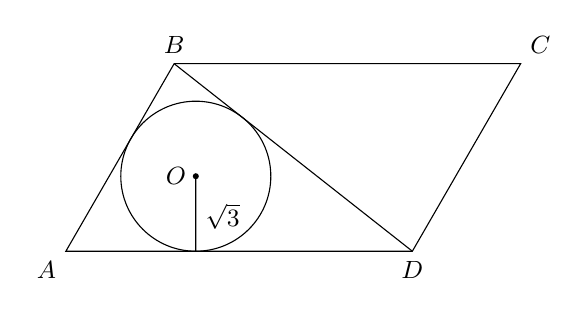
\begin{tikzpicture}[scale=0.55,font=\small]
\coordinate (A) at (0,0); \coordinate (D) at (8,0); \coordinate (B) at (2.5,4.33); \coordinate (C) at (10.5,4.33); \coordinate (O) at (3,1.732);
\draw (A)--(B)--(C)--(D)--cycle; \draw (B)--(D); \draw (O) circle (1.732); \draw (O)--(3,0); \fill (O) circle (2pt);
\node[below left] at (A) {$A$}; \node[above] at (B) {$B$}; \node[above right] at (C) {$C$}; \node[below] at (D) {$D$}; \node[left] at (O) {$O$}; \node[right] at (3,0.8) {$\sqrt3$};
\end{tikzpicture}}
\AB{Parallelogramm yuzini toping.}{Parallelogrammning katta tomonini toping.}}
\QQ{43}{Muntazam ön ikkiburçakning tomoni $\sqrt3-1$ ga teng.
\qfig{\begin{tikzpicture}[scale=1.4,font=\small]
\foreach \n/\a in {A/105,B/75,C/45,D/15,E/-15,F/-45,G/-75,H/-105,I/-135,J/-165,K/165,L/135} {\coordinate (\n) at (\a:1); \node at (\a:1.17) {$\n$};}
\fill[qfill] (L)--(E)--(F)--cycle;
\draw (A)--(B)--(C)--(D)--(E)--(F)--(G)--(H)--(I)--(J)--(K)--(L)--cycle; \draw (L)--(C); \draw (L)--(E); \draw (L)--(F);
\end{tikzpicture}}
\AB{$|LC|$ ni toping.}{$LEF$ böyalgan soha yuzasini toping.}}
\QQ{44}{Radiusi $R$ ga teng bölgan yarim aylana berilgan. Undan konus yasaldi.
\qfig{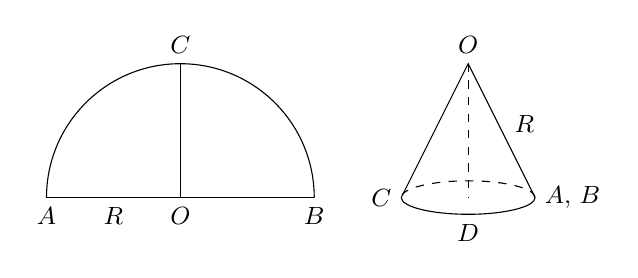
\begin{tikzpicture}[scale=0.85,font=\small]
\draw (-2,0)--(2,0); \draw (2,0) arc (0:180:2); \draw (0,0)--(0,2);
\node[below] at (-2,0) {$A$}; \node[below] at (2,0) {$B$}; \node[below] at (0,0) {$O$}; \node[above] at (0,2) {$C$}; \node[below] at (-1,0) {$R$};
\begin{scope}[xshift=4.3cm]
\coordinate (O) at (0,2); \coordinate (C) at (-1,0); \coordinate (AB) at (1,0);
\draw (C)--(O)--(AB); \draw (C) arc (180:360:1 and 0.25); \draw[dashed] (AB) arc (0:180:1 and 0.25); \draw[dashed] (O)--(0,0);
\node[above] at (O) {$O$}; \node[left] at (C) {$C$}; \node[right] at (AB) {$A,\,B$}; \node[right] at (0.55,1.1) {$R$}; \node[below] at (0,-0.25) {$D$};
\end{scope}
\end{tikzpicture}}
\AB{Konus yasovçisi va öqi orasidagi burçakning sinusini toping.}{$R=2\sqrt3$ bölsa, konusga içki çizilgan sfera sirtining yuzini toping. ($\pi\approx3$ deb oling)}}
\QQ{45}{Kema harakatga kelişi uçun işçilarga va yoqilğiga pul sarflaydi. Işçilarga soatiga $250$ \$ dan, yoqilği uçun esa soatiga $v^3$ \$ pul sarflaydi. Kemaning örtaça tezligi $v$ (km/h) ga teng.
\AB{Agar $10$ km masofani bosib ötiş uçun eng kam pul sarflansa, $v$ (km/h) ni toping.}{$10$ km masofani bosib ötiş uçun eng kam qança harajat sarflanadi?}}
\Javoblar{A B D A D C A D D A C A A B A A B B A D A A B D A A A A C C D A B E C}{%
\OK{36}{$4$}{$7$}\OK{37}{$2$}{$\dfrac{\sqrt{10}}2$}\OK{38}{$1$}{$15$}\OK{39}{$-3$}{$-5$}\OK{40}{$2\sqrt5$}{$\dfrac43$}%
\OK{41}{$5\sqrt2$}{$5$}\OK{42}{$20\sqrt3$}{$8$}\OK{43}{$2$}{$1$}\OK{44}{$\dfrac12$}{$12$}\OK{45}{$5$}{$750$}}
